%File: functional-data.tex
%Date: Sat Oct 19 17:10:24 2013 +0800
%Author: Xinyu Zhou <zxytim@gmail.com>

\subsection{Data Management}

\subsubsection{Items}

An item is piece of information retrieved from various sources, and
shown in lists for further reading. It consists of following parts:

\begin{itemize}
\itemsep1pt\parskip0pt\parsep0pt
\item
  Title
\item
  Source
\item
  Content
\item
  Labels
\item
  Comments
\end{itemize}

Item is the core entity in Uknow system. A user can manipulate items in
following ways:

\begin{description}
\item[Removal] \hfill

  When a user find a specific item unpleasant, unattractive or redundant, he/she
  may remove this item using the button provided, as shown in \figref{delete}. Removal operation can be
  reversed within a short period of time to prevent from mis-clicking the button.

\begin{figure}[H]
  \centering
  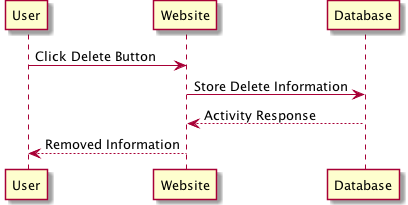
\includegraphics[width=0.6\textwidth]{img/delete.png}
  \caption{Removal process\label{fig:delete}}
\end{figure}


\item[Archive] \hfill

  User can store specific items for further reading or recapping in
  the future. Archived items still show up in item flow, and will be
  labeled as `archived'.

\item[Share] \hfill

  If an item fascinates a user, he/she may share it among popular SNS.
  When first sharing an item, user will authenticate its account on
  desired SNS website, and after confirmation, a sharing information
  will be posted on the chosen SNS.

\item[Like] \hfill

  Users can show theirs preferences on certain items, and others will
  know the statistics, and this could be used as an score to evaluate an
  item. For a better reading experience, high score items are more likely to rank higher in the item flow than low score items.

\item[Comment] \hfill

  Users can post comments under an item. Posts will be stored in
  this system, and can optionally be posted synchronously on item
  source, if the source website supports such functionality.

  Comments is organized hierarchically. If a user intends to reply
  other's comment, he/she can click the reply button, and the
  reply form should show right below the comment.

  When complete typing, click the reply button and the comments shall be
  posted, and the form will consequently disappear.
\end{description}

Furthermore, system can learn from user behaviors on items and to
recommend items related to users' interest.

\subsubsection{Labels}

A label is an attribute describing items. An item can have multiple
labels. A label associated with an item may be automatically assigned by
system, or tagged by users. A label can be either a system-wide label,
which is visible to all user, or a user specified label which indicates
user preferences on an item.

Label may come from:

\begin{description}
\item[System Pre-tagging]
  An item may arrive to a user with pre-tagged
  labels. These pre-tagged labels are vital to subsequent data
  processing, such as tag-filtering plugins in tabs.

\item[User-tagging]
  Same item could have distinct meaning to different user.
  User can tag item with labels cater to their taste, as well as remove
  labels that could lead to misunderstanding to itself, as shown in \figref{tagging}.

\begin{figure}[H]
  \centering
  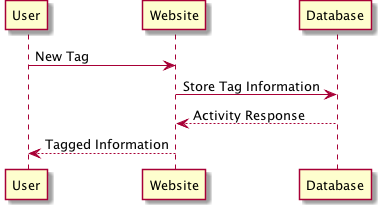
\includegraphics[width=0.6\textwidth]{img/tagging.png}
  \caption{Tagging process\label{fig:tagging}}
\end{figure}

\end{description}

As described aforementioned, functions like `archive' is actually a process of tagging an
item by the label `archived'

\subsubsection{Plugins}

Plugin is an essential concept in Uknow system, which comprises the
implementations of varied functionalities in the system. A plugin should
process a bunch of items, returning processed items. The number of items
before and after need not to be the same, that is, a plugin can either
shrink items or enrich items (filtering job) or process on contents of
items.

User can choose a subset of provided plugins to employ on its items.
Plugin can be either scoped to a `tab' or can be applied system-wide.

Plugins can be configurable, but configuration is plugin-dependent.

Examples of plugins:

\begin{description}
\item[Tag-filtering] Allowing users to choose preferred tags.
\item[Highlight] Highlight significant words in an item.
\item[Emotion tagging] Detect emotion of an item.
\item[Face detection in image] Detect faces from images of an item.
\item[Related items] Recommend related items for users to discover new contents to read.
\end{description}

\subsubsection{Tabs}

Tab is a collection of filtered items, in which the filter is defined by
plugins. A typical use of tab is to divide items into different
categories, which can be exclusive or not.

Tabs can be added or removed on-the-fly with `add' or `remove' button,
add define its behaviour with plugins.

Moreover, tab layout, item flow style, etc., are also configurable via
tab configuration.
